\section{Optoelectronic coupling}

The noninteracting system displays valley selective optical excitations. Light
of a particular polarity only couples to one valley. Since the superconducting state is
a coherent condensate admixing the two valleys, the question we address is whether pair breaking
also displays valley selectivity. In particular we explore whether or not the two quasiparticles generated
by circularly polarized light, with total energy larger than the $\Delta+\Delta _{\vec{k}}$, occupy opposite
valleys, with one in the conduction band and the other in the valence band.

The optical excitations arise from the Berry curvature,
which acts as an effective angular momentum.
The electromagnetic potential $\vc{A}$,
with polarization vector $\vc{ϵ}$,
is introduced using minimal coupling,
$H_{τ {\s}}^{ν ν'} \ofK
→ H_{τ {\s}}^{ν ν'} \of{\vK + e \vc{A}}$,
where, in the dipole approximation,
$\vc{A} = 2 \re{\vc{ϵ} A_0 e^{- i ω t}}$.
This yields a perturbed Hamiltonian
$H → H + H^A$, where
$H^A = H' e^{- i ω t} + H'^† e^{i ω t}$,
with
\begin{multline}
  H'
  = ∑_{\vK, τ, {\s}}
    H'_τ
    {d^-_{τ {\s}}}^† \ofK
    d^+_{τ {\s}} \ofK \\
  - ∑_{\vK, τ, {\s}}
    H'_{-τ}
    {d^+_{τ {\s}}}^† \ofK
    d^-_{τ {\s}} \ofK,
\end{multline}
and
$H'_τ
= a t e A_0
\left( τ \vc{\hat{x}} + i \vc{\hat{y}} \right) · \vc{ϵ}$.
The transition rate is proportional to the modulus-squared
of the optical matrix elements,
$\vc{P}_{τ {\s}}^{n n'} \ofK$,
defined by
\begin{equation}
  H^A
  = ∑_{\substack{\vK, τ, {\s} \\ n, n'}}
    \frac{e A_0}{m_0}
    \vc{ϵ} · \vc{P}_{τ {\s}}^{n n'} \ofK
    {c_{τ {\s}}^n}^† \ofK
    c_{τ {\s}}^{n'} \ofK.
\end{equation}
For circularly polarized light, in the absence of superconductivity,
$\vc{ϵ}_± = \left( \vc{\hat{x}} ± i \vc{\hat{y}} \right) / \sqrt{2}$ and
\begin{equation}
  \label{eq:optical}
  \vc{ϵ}_± · \vc{P}_{τ {\s}}^{+ -} \of{\vK}
  = ∓ τ \sqrt{2} a t m_0
    e^{± i ϕ}
    \sin^2 {\frac{\fnTheta{∓ τ}}{2}}.
\end{equation}

The transition rate for optical excitations from BCS ground state
is given by \cref{eq:optical}
multiplied by a coherence factor $\sin^2 {β_{\vK}}$.
Since $\fnTheta{-} - \fnTheta{+} = τ π$,
switching either the valley or polarization transforms
$\sin → \cos$ in \cref{eq:optical}, giving matrix elements,
$\left| P_± \right| = \left| \vc{ϵ}_± · P_+^{+ -} \sin {β} \right|$,
corresponding to matching ($P_+$) or mismatching ($P_-$)
polarization-valley indexes.

\begin{figure}
  \caption{}
  \begin{subfigure}{\columnwidth}
    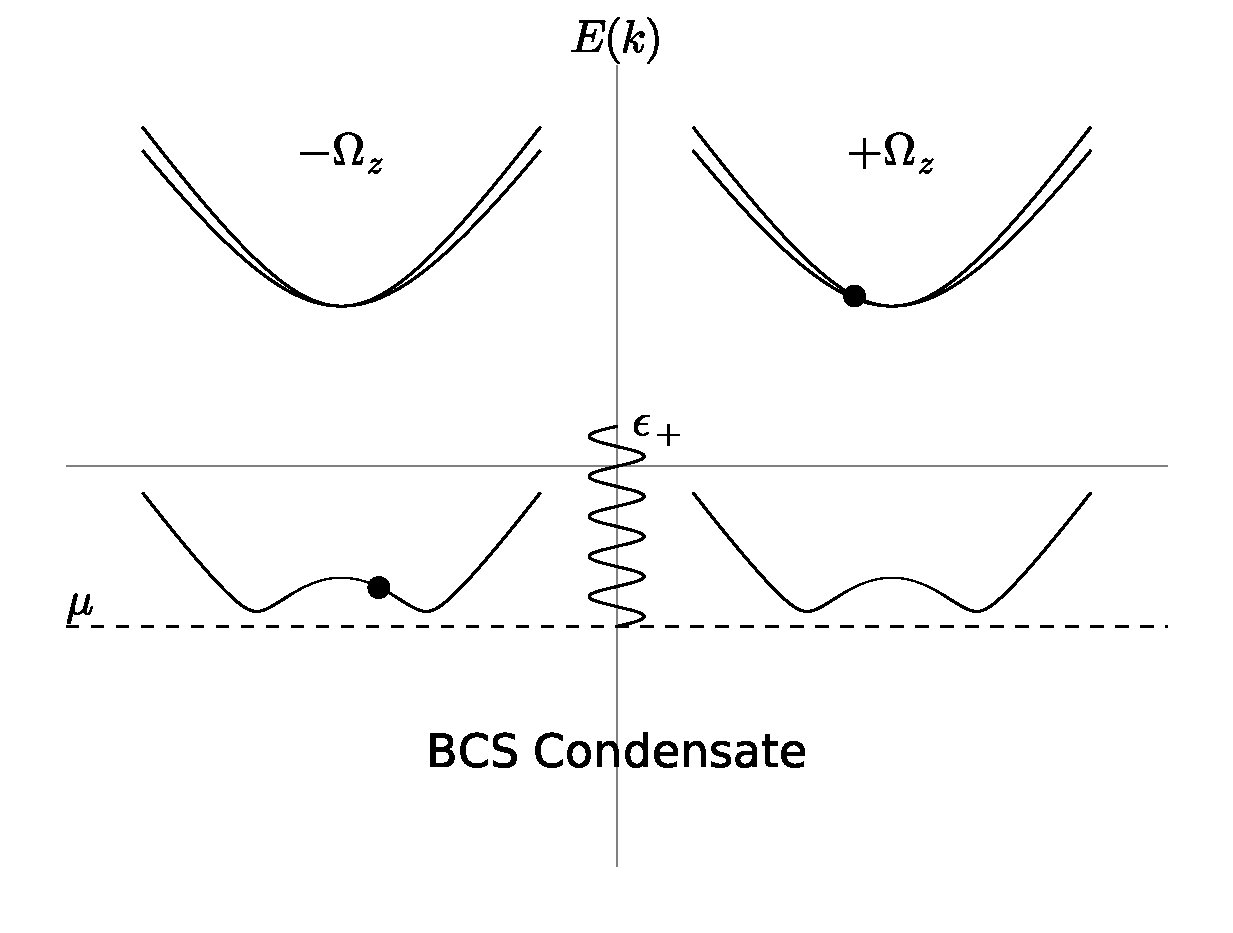
\includegraphics[width=\columnwidth]{figures/bcs-excitation}
    \caption{%
      Pair breaking by right circularly polarized light leads to an electron in the conduction band of the right valley
      and a partner in the valence band of the left valley. The valleys interchange for left circularly polarized light.
    }\label{fig:optical-excitation}
  \end{subfigure}
  \begin{subfigure}{\columnwidth}
    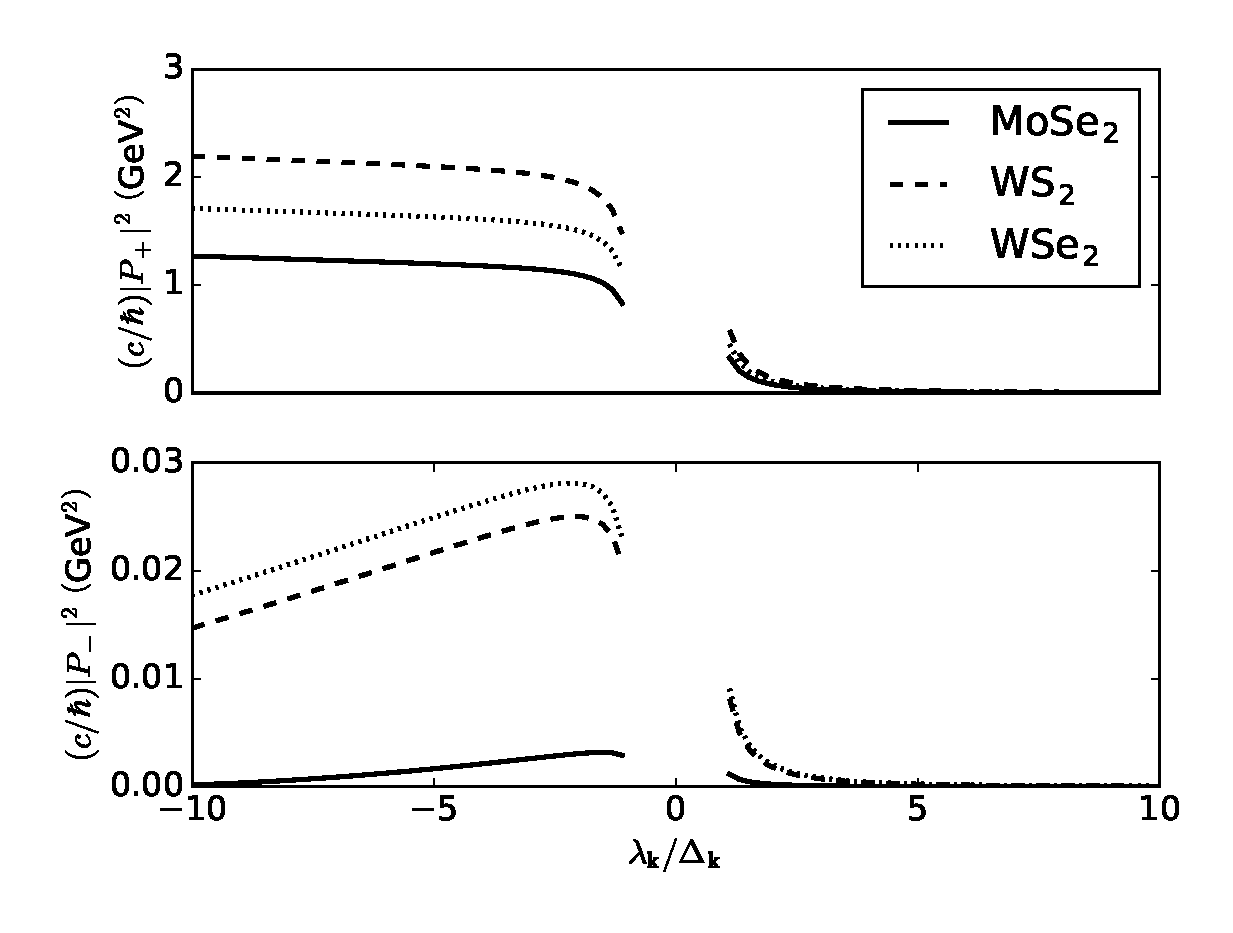
\includegraphics[width=\columnwidth]{figures/optical-transitions}
    \caption{%
      Optical transition rate matrix elements
      $\left| P_± \right|^2$
      in the superconducting phase
      as a function of the ratio of the quasiparticle energy
      $λ_{\vK}$ to the superconducting gap $Δ_{\vK}$.
      Material parameters for \ce{MoSe2}, \ce{WS2}, and \ce{WSe2}
      are given in~\cite{PhysRevLett.108.196802}
      and a gap of $Δ_{\vK} = \SI{7.5}{\milli\electronvolt}$
      is chosen for illustrative purposes.
      The order-of-magnitude contrast between
      $\left|P_+\right|^2$ and $\left|P_-\right|^2$
      causes the optical-valley selectivity.
    }\label{fig:optical}
  \end{subfigure}
\end{figure}

For a given valley, a chosen polarization of light couples more strongly
than the other, as is evident comparing $\abs{P_+}^2$ to $\abs{P_-}^2$
and shown in \cref{fig:optical}. For incident light with energy $\Delta + |\lambda_{\vc{k}}|$,
right circurlalrly polarized light (+) has a higher probability of promoting a quasiparticle to the
conduction band as reflected in larger matrix element $|P_{+}|^{2}>>|P_{-}|^{2}$. The partner of the copper
pair is in the valence band in the opposite valley. The dependance on polarization
is opposite in the other valley.

This is a key new result and opens the door for valley control of excitations
from a coherent ground state. For example, the two quasiparticles have the same Berry curvature (see below) and charge.
In the presence of an electric filed, they both acquire the same transverse anomalous velocity. Thus an anomalous Hall effect
is anticipated, with no accompanying spin current in contrast to the response in the normal state.
